\documentclass[aspectratio=169]{beamer}

\usetheme{Boadilla}
\usefonttheme{professionalfonts}
\setbeamertemplate{navigation symbols}{}
\setbeamertemplate{itemize items}[circle]
\setbeamertemplate{enumerate items}[default]
\setbeamertemplate{headline}{}

\usepackage[utf8]{inputenc}
\usepackage[T1]{fontenc}
\usepackage{lmodern}
\usepackage{amsmath}
\usepackage{booktabs}
\usepackage{tabularx}
\usepackage{array}
\usepackage{hyperref}
\usepackage[strings]{underscore}
\usepackage{listings}
\usepackage{tikz}
\usetikzlibrary{arrows.meta,positioning,fit,calc,shapes.geometric}
\usepackage{xcolor}

\definecolor{courseblue}{HTML}{12355B}
\definecolor{coursegold}{HTML}{C98A2E}
\definecolor{courseice}{HTML}{EEF3F8}
\definecolor{coursegreen}{HTML}{2F6B4F}
\definecolor{coursegray}{HTML}{4B5563}
\definecolor{codebg}{HTML}{F7F9FC}
\definecolor{codecomment}{HTML}{5E6C84}
\definecolor{codestring}{HTML}{0B6E4F}

\setbeamercolor{palette primary}{bg=courseblue,fg=white}
\setbeamercolor{palette secondary}{bg=coursegold,fg=white}
\setbeamercolor{palette tertiary}{bg=courseblue,fg=white}
\setbeamercolor{palette quaternary}{bg=coursegold,fg=white}
\setbeamercolor{structure}{fg=courseblue}
\setbeamercolor{frametitle}{bg=courseice,fg=courseblue}
\setbeamercolor{title}{fg=courseblue}
\setbeamercolor{block title}{bg=courseblue,fg=white}
\setbeamercolor{block body}{bg=courseice,fg=black}
\setbeamercolor{normal text}{fg=black,bg=white}
\setbeamercolor{alerted text}{fg=coursegold}

\setbeamerfont{footline}{size=\scriptsize}

\setbeamertemplate{footline}{
  \leavevmode
  \hbox{
    \begin{beamercolorbox}[wd=.33\paperwidth,ht=2.8ex,dp=1.2ex,leftskip=0.8em]{palette primary}%
      University of Trieste
    \end{beamercolorbox}%
    \begin{beamercolorbox}[wd=.49\paperwidth,ht=2.8ex,dp=1.2ex,center]{palette tertiary}%
      \coursename{} \textbar{} \coursecode
    \end{beamercolorbox}%
    \begin{beamercolorbox}[wd=.18\paperwidth,ht=2.8ex,dp=1.2ex,rightskip=0.8em plus1fil]{palette secondary}%
      \insertframenumber{} / \inserttotalframenumber
    \end{beamercolorbox}%
  }
}

\hypersetup{
  colorlinks=true,
  linkcolor=courseblue,
  urlcolor=coursegreen
}

\lstdefinestyle{coursepython}{
  language=Python,
  basicstyle=\ttfamily\footnotesize,
  keywordstyle=\color{courseblue}\bfseries,
  commentstyle=\color{codecomment}\itshape,
  stringstyle=\color{codestring},
  showstringspaces=false,
  columns=fullflexible,
  keepspaces=true,
  frame=single,
  framerule=0.6pt,
  rulecolor=\color{courseblue},
  backgroundcolor=\color{codebg},
  xleftmargin=0.4em,
  xrightmargin=0.4em,
  aboveskip=0.4em,
  belowskip=0.2em
}

\newcommand{\coursename}{Data-driven Systems Engineering}
\newcommand{\coursecode}{440MI / 305SM}
\newcommand{\coursefooter}{}

\newcommand{\learninggoals}[1]{
  \begin{block}{Learning goals}
  #1
  \end{block}
}

\newcommand{\repoactivity}[1]{
  \begin{block}{Repo activity}
  #1
  \end{block}
}

\newcommand{\readinglist}[1]{
  \begin{block}{Papers and materials}
  {\footnotesize #1}
  \end{block}
}

\newcommand{\coursecontextframe}[5]{
  \begin{frame}{Course Map and Running Cases}
  \centering
  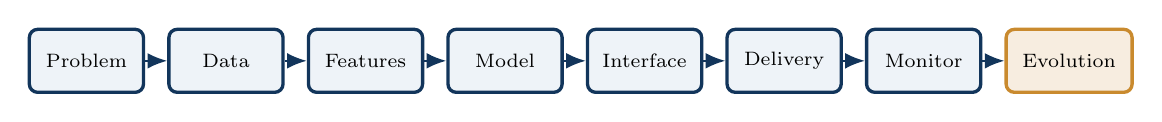
\begin{tikzpicture}[node distance=0.28cm]
  \node[flowbox, minimum width=1.45cm, minimum height=0.8cm] (problem) {\scriptsize Problem};
  \node[flowbox, minimum width=1.45cm, minimum height=0.8cm, right=of problem] (data) {\scriptsize Data};
  \node[flowbox, minimum width=1.45cm, minimum height=0.8cm, right=of data] (features) {\scriptsize Features};
  \node[flowbox, minimum width=1.45cm, minimum height=0.8cm, right=of features] (model) {\scriptsize Model};
  \node[flowbox, minimum width=1.45cm, minimum height=0.8cm, right=of model] (interface) {\scriptsize Interface};
  \node[flowbox, minimum width=1.45cm, minimum height=0.8cm, right=of interface] (delivery) {\scriptsize Delivery};
  \node[flowbox, minimum width=1.45cm, minimum height=0.8cm, right=of delivery] (monitor) {\scriptsize Monitor};
  \node[accentbox, minimum width=1.6cm, minimum height=0.8cm, right=of monitor] (evolution) {\scriptsize Evolution};
  \foreach \a/\b in {problem/data,data/features,features/model,model/interface,interface/delivery,delivery/monitor,monitor/evolution} {
    \draw[arrow] (\a) -- (\b);
  }
  \end{tikzpicture}

  \vspace{0.5em}
  \begin{block}{Today in the course}
  \textbf{Focus:} #1

  \textbf{Bridge:} #2
  \end{block}

  \begin{columns}[T]
  \column{0.48\textwidth}
  \begin{block}{Fraud case}
  {\footnotesize #3}
  \end{block}
  \column{0.48\textwidth}
  \begin{block}{Pasteurization case}
  {\footnotesize #4}
  \end{block}
  \end{columns}

  \vspace{0.3em}
  {\footnotesize \textbf{Course thread:} #5}
  \coursefooter
  \end{frame}
}

\newcommand{\classclosingframe}[4]{
  \begin{frame}{From This Class to the Next}
  \begin{block}{What stays with us}
  #1
  \end{block}

  \begin{columns}[T]
  \column{0.48\textwidth}
  \begin{block}{Project use}
  {\footnotesize #2}
  \end{block}
  \column{0.48\textwidth}
  \begin{block}{Next connection}
  {\footnotesize #3}
  \end{block}
  \end{columns}

  \vspace{0.3em}
  {\footnotesize \textbf{Course thread:} #4}
  \coursefooter
  \end{frame}
}

\tikzset{
  flowbox/.style={
    rounded corners=3pt,
    draw=courseblue,
    fill=courseice,
    very thick,
    minimum width=2.2cm,
    minimum height=0.9cm,
    align=center,
    font=\small
  },
  accentbox/.style={
    rounded corners=3pt,
    draw=coursegold,
    fill=coursegold!15,
    very thick,
    minimum width=2.2cm,
    minimum height=0.9cm,
    align=center,
    font=\small
  },
  arrow/.style={
    -{Latex[length=2.5mm,width=2mm]},
    thick,
    draw=courseblue
  }
}


\title{Class 31: Continuous Monitoring and Scalability}
\subtitle{Session 31 of 36 -- MLOps Block}
\author{\coursename}
\date{}

\begin{document}

\frame{\titlepage \coursefooter}

\begin{frame}{Agenda}
\begin{itemize}
\item Why monitoring matters
\item Monitoring as risk control, and monitoring types
\item Data drift versus concept drift, and detection strategies
\item Response after alerts
\item Scalability: load, horizontal scaling, and cost-latency trade-offs
\end{itemize}
\coursefooter
\end{frame}

\begin{frame}{Monitoring and scaling turn deployment into an ongoing job}
\learninggoals{
\begin{itemize}
\item Distinguish system, data, model, and business monitoring layers.
\item Compare data drift, concept drift, and pipeline failure symptoms.
\item Design practical responses after a drift alert.
\item Reason about load, horizontal scaling, and cost-latency trade-offs for serving ML systems.
\end{itemize}
}
\coursefooter
\end{frame}

\coursecontextframe
{Monitoring, drift response, and scaling under real load.}
{This class extends delivery into sustained operation: a shipped system must stay correct as data drifts and stay responsive as traffic grows.}
{In the fraud case, monitoring covers data shift, score behavior, and analyst workload, while scaling covers what happens to latency during a transaction spike.}
{In the pasteurization case, monitoring covers sensor quality and state transitions, while scaling covers serving many simultaneous plant dashboards from one stream.}
{Observation and scale are where an engineered system proves itself over time; the course now carries this into project execution.}

\begin{frame}{Why monitoring matters}
\begin{itemize}
\item ML systems are data products, not static binaries.
\item Degradation can be silent and expensive.
\item Labels may arrive late, so proxies matter.
\item Monitoring is evidence for operations, governance, and improvement.
\end{itemize}
\coursefooter
\end{frame}

\begin{frame}{Monitoring is quantified risk management}
\begin{itemize}
\item Data risk: changed distributions, missing features, schema violations.
\item Model risk: degraded performance, instability, concept drift, unfairness.
\item Operational risk: broken pipelines, latency spikes, failed endpoints.
\item Business risk: review overload, poor intervention yield, loss of trust.
\end{itemize}
\begin{block}{Meaning}
Monitoring turns hidden failure into visible evidence that teams can act on.
\end{block}
\coursefooter
\end{frame}

\begin{frame}{What should be monitored in an ML service?}
\centering
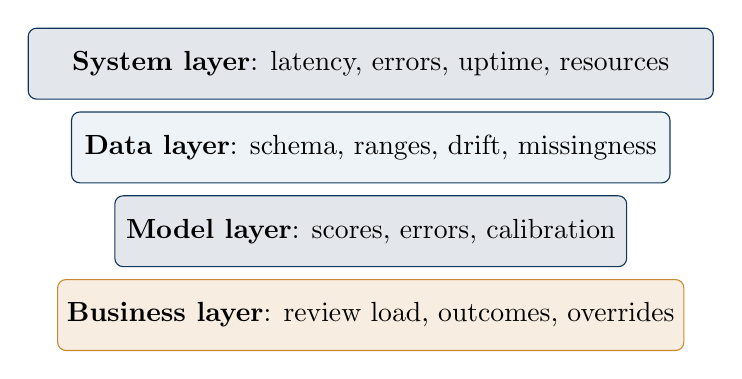
\begin{tikzpicture}[node distance=0.15cm]
\node[draw=courseblue, fill=courseblue!12, rounded corners=3pt, minimum width=8.7cm, minimum height=0.9cm] (system) {\textbf{System layer}: latency, errors, uptime, resources};
\node[draw=courseblue, fill=courseice, rounded corners=3pt, minimum width=7.6cm, minimum height=0.9cm, below=of system] (data) {\textbf{Data layer}: schema, ranges, drift, missingness};
\node[draw=courseblue, fill=courseblue!12, rounded corners=3pt, minimum width=6.5cm, minimum height=0.9cm, below=of data] (model) {\textbf{Model layer}: scores, errors, calibration};
\node[draw=coursegold, fill=coursegold!15, rounded corners=3pt, minimum width=5.4cm, minimum height=0.9cm, below=of model] (biz) {\textbf{Business layer}: review load, outcomes, overrides};
\end{tikzpicture}
\coursefooter
\end{frame}

\begin{frame}{Data drift vs concept drift}
\begin{itemize}
\item Data drift: input distribution changes, even if the relationship still holds.
\item Concept drift: the mapping from input to target changes.
\item Pipeline bugs can mimic both and must be ruled out early.
\end{itemize}
\begin{block}{Examples}
Holiday shopping patterns can cause fraud feature drift; a new attack strategy can create concept drift.
\end{block}
\coursefooter
\end{frame}

\begin{frame}{What can look like drift but is not}
\begin{itemize}
\item A broken ingestion job that changes missing-value rates.
\item A schema change that reorders or renames columns.
\item A deployment mismatch between training preprocessing and live preprocessing.
\item A monitoring bug that changes the way metrics are computed.
\end{itemize}
\begin{block}{Rule}
Before retraining, verify that the problem is real and not a pipeline defect.
\end{block}
\coursefooter
\end{frame}

\begin{frame}{Detection strategies}
\begin{itemize}
\item Batch statistical tests: KS, PSI, chi-square, Jensen-Shannon variants.
\item Prediction monitoring: score distribution and confidence shifts.
\item Label-based metrics when ground truth arrives.
\item Streaming detectors: ADWIN, Page-Hinkley, DDM, EDDM.
\end{itemize}
\coursefooter
\end{frame}

\begin{frame}{A practical drift-detection taxonomy}
\begin{tabularx}{\textwidth}{>{\bfseries}l X}
Signal type & Typical use \\
\toprule
Feature distribution tests & Early warning when labels are delayed. \\
Prediction distribution checks & Detect score collapse or threshold instability. \\
Label-based performance & Confirm concept drift when outcomes arrive. \\
Streaming detectors & Catch online change in error or metric sequences. \\
Segment analysis & Reveal that drift affects only some populations. \\
\bottomrule
\end{tabularx}
\coursefooter
\end{frame}

\begin{frame}[fragile]{Repository-style online monitoring loop}
\begin{lstlisting}[style=coursepython]
y_pred = model.predict_one(x)
model.learn_one(x, y)
mae.update(y, y_pred)
error = abs(y - (y_pred or 0))
adwin.update(error)
drift_flag = adwin.drift_detected
\end{lstlisting}
\begin{itemize}
\item `streamlit/pages/App_Stream.py` uses this pattern to combine incremental learning, error tracking, and ADWIN-based change detection.
\item It is useful because the alert is tied to live behavior, not only offline charts.
\end{itemize}
\coursefooter
\end{frame}

\begin{frame}{Repo examples for a stronger lecture}
\repoactivity{
\begin{itemize}
\item `streamlit/pages/App_Stream.py` already combines online learning with ADWIN.
\item `documents/Forecasting_and_Drift_Pasteurization.pdf` defines a project around forecasting and drift detection.
\item `pasteurization/synth_sensors.py` gives state-aware signals for meaningful monitoring discussions.
\item `pasteurization/serving.py` is also our only in-repo example of a streaming service under simulated load.
\end{itemize}
}
\coursefooter
\end{frame}

\begin{frame}{After detection: diagnose, then respond}
\begin{enumerate}
\item Verify the alert is not caused by ingestion or schema issues.
\item Diagnose whether the change is temporary, seasonal, or structural.
\item Choose a response: retrain, recalibrate, switch model, roll back, add human review, or change thresholds.
\item Record the event for later audit and process learning.
\end{enumerate}
\coursefooter
\end{frame}

\begin{frame}{Performance over time and business metrics}
\begin{itemize}
\item Model metrics: accuracy, precision, recall, AUC, MAE, RMSE.
\item Operational metrics: latency, queue length, failed predictions.
\item Business metrics: intervention yield, review load, false alert fatigue.
\item Human signals: overrides, complaints, and trust breakdowns.
\end{itemize}
\coursefooter
\end{frame}

\begin{frame}{Champion-challenger and continuous comparison}
\begin{itemize}
\item A champion model serves production traffic.
\item A challenger runs in shadow mode or on sampled traffic.
\item Comparison over time helps avoid switching on the basis of one lucky offline result.
\item This strategy is especially useful when concept drift is suspected but labels are delayed.
\end{itemize}
\coursefooter
\end{frame}

\begin{frame}{From watching the system to sizing it}
\begin{itemize}
\item Monitoring tells us the system is behaving correctly; scalability asks whether it keeps behaving correctly under more load.
\item Load can grow in requests per second, batch size, number of streams, or number of simultaneous dashboards.
\item A model that is accurate but too slow or too expensive under load is still a failed system.
\end{itemize}
\coursefooter
\end{frame}

\begin{frame}{Horizontal scaling for a serving layer}
\centering
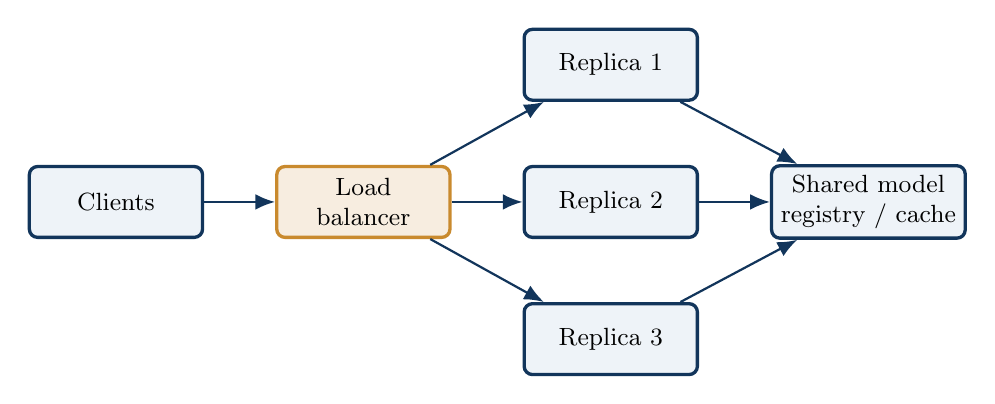
\begin{tikzpicture}[node distance=0.8cm and 0.9cm]
\node[flowbox] (client) {Clients};
\node[accentbox, right=of client] (lb) {Load\\balancer};
\node[flowbox, above right=of lb] (r1) {Replica 1};
\node[flowbox, right=of lb] (r2) {Replica 2};
\node[flowbox, below right=of lb] (r3) {Replica 3};
\node[flowbox, right=of r2] (store) {Shared model\\registry / cache};
\draw[arrow] (client) -- (lb);
\draw[arrow] (lb) -- (r1);
\draw[arrow] (lb) -- (r2);
\draw[arrow] (lb) -- (r3);
\draw[arrow] (r1) -- (store);
\draw[arrow] (r2) -- (store);
\draw[arrow] (r3) -- (store);
\end{tikzpicture}
\vspace{0.5em}
\begin{itemize}
\item Stateless replicas behind a load balancer are the standard pattern; each replica loads the same versioned artifact from a shared registry.
\item Autoscaling adds or removes replicas based on load signals such as queue depth or CPU.
\end{itemize}
\coursefooter
\end{frame}

\begin{frame}{Cost-latency trade-offs when scaling ML services}
\begin{tabularx}{\textwidth}{>{\bfseries}l X}
Lever & Trade-off \\
\toprule
More replicas & Lower latency under load, higher infrastructure cost. \\
Smaller batch size & Lower per-request latency, lower throughput per instance. \\
Bigger instance type & Handles larger models, higher idle-time cost. \\
Prediction caching & Cuts recompute for repeated inputs, risks staleness. \\
Async or queued inference & Smooths spikes, adds response delay. \\
\bottomrule
\end{tabularx}
\coursefooter
\end{frame}

\begin{frame}{Practical Component}
\begin{block}{Honest gap in this repository}
There is currently no in-repo monitoring dashboard or load-testing exercise beyond the basic streaming demo in `pasteurization/serving.py`.
\end{block}
\begin{itemize}
\item A drift-alert dashboard, or a simple load test against the Flask or streaming endpoints, does not yet exist as a repo exercise.
\item This is suggested as a separate project, for example a dedicated GitHub submodule, rather than invented here.
\item Until it exists, this class stays conceptual: reason about the trade-offs, sketch the architecture, but do not pretend a working benchmark is already in the repo.
\end{itemize}
\coursefooter
\end{frame}

\begin{frame}{Discussion prompt}
\begin{block}{Question}
The fraud API is correct and well-monitored at 10 requests per second. What is the first thing likely to break at 10,000, and how would you know before it happens in production?
\end{block}
\begin{itemize}
\item This connects monitoring evidence to scaling decisions instead of treating them as separate topics.
\item It also motivates load testing as a form of validation, not only a performance nice-to-have.
\end{itemize}
\coursefooter
\end{frame}

\begin{frame}{Papers and materials}
\readinglist{
\href{https://riverml.xyz/latest/api/drift/ADWIN/}{River ADWIN documentation};\
\href{https://www.oreilly.com/library/view/practical-mlops/9781098103002/}{Practical MLOps};\
\href{https://www.oreilly.com/library/view/reliable-machine-learning/9781098106218/}{Reliable Machine Learning};\
\href{https://arxiv.org/abs/2007.06299}{Gama et al., A survey on concept drift adaptation};\
\href{https://evidentlyai.com/blog/data-drift-detection-large-datasets}{Evidently on data drift detection};\
\href{https://prometheus.io/docs/introduction/overview/}{Prometheus monitoring overview};\
\href{https://12factor.net/}{The Twelve-Factor App, on stateless, horizontally scalable services}.
}
\coursefooter
\end{frame}

\classclosingframe
{\begin{itemize}
\item Monitoring turns deployment into an ongoing feedback process instead of an endpoint.
\item Drift detection matters only when the team has diagnosis and response mechanisms.
\item Scalability is a system property to design for, not a surprise to react to after launch.
\end{itemize}}
{For both running cases, long-term value depends on observing data quality, model behavior, and operational health, and on knowing how the system behaves under more load than a demo ever sees.}
{Class 32 turns this full lifecycle view into a working session where teams scope their own capstone project.}
{Every architecture, feature, model, interface, and process choice in this course should support sustainable evolution under real, growing use.}

\end{document}
